\documentclass{assignment-263}

\usepackage{color}

\usepackage{mathtools}
\anum{3}
\course{CSC263}
\duedate{Monday, March 30, 2020}
\filename{ps3.pdf, ps3.tex and cities.py}

\newcommand{\bigOh}{\mathcal{O}}

\begin{document}
\think

  \begin{enumerate}[1.]

\item \textbf{Number of Shortest Paths [total: 10]}
Let $G = (V ,E)$ be a unweighted directed connected graph. Design an algorithm that determines for two given nodes $s, t \in V$ the number of shortest paths from $s$ to $t$ in $O(|V| + |E|)$. 
\begin{enumerate}[(a)]
\item Write your algorithm in pseudocode and describe its functionality in concise (but precise) English.
\item Prove the correctness and runtime of your algorithm in Part 1a.
\end{enumerate}

\item \textbf{MST [total: 8]} 
Let $G = (V ,E)$ be a weighted undirected connected graph that
contains a cycle, and let $e$ be a maximum-weight edge among all edges in the cycle. Prove that there exists a minimum spanning tree of $G$ which does NOT include $e$.


\item \textbf{Catch the Human [total: 10]}
  In a rectangular field with \texttt{m} by \texttt{n} squares there is a human \textbf{H} and two robots \textbf{R1} and \textbf{R2} (see Figure~\ref{fig:map}). 
  Each of the three starts off at some initial square.
  At the beginning of the game, \textbf{H, R1, R2}, all know each
  other's positions. 

  Each turn, the \textbf{H} makes the first move, followed by \textbf{R1} and \textbf{R2}. 
  A move can be either exactly one square up, down, left, or right (or
  can choose to stay at their current location).
  Grey squares are inaccessible as they mark obstacles.
  If \textbf{R1} or \textbf{R2} can move to the same square which \textbf{H} is on, they catch \textbf{H}.

  In order to escape, at the beginning of the game, before the first
  turn, \textbf{H must declare} a single square \textbf{Y}
  (e.g. $(3,1)$) at the edge of the field (the yellow zone) that the
  human is going to reach for. If \textbf{H} reaches the square
  \textbf{Y}, it is able to escape at its next turn if it is not
  caught by \textbf{R1} or \textbf{R2} before that. Otherwise,
  \textbf{H} is unable to escape.

  Note that the game can end only at the end of a full turn. So in an
  example scenario where: 1) \textbf{Y} is empty before a turn, 2)
  \textbf{H} makes its next move and reaches \textbf{Y}, 3)
  \textbf{R1} makes its next move and reaches \textbf{Y};  \textbf{H}
  gets caught and is unable to escape.
  
  % If \textbf{H} is standing in a square at the edge of the field (the yellow zone), then in the next turn \textbf{H} can jump off the field and safely escape from \textbf{R1}'s and \textbf{R2}'s chase.

  
  \begin{figure}[!h]
  	\centering
  	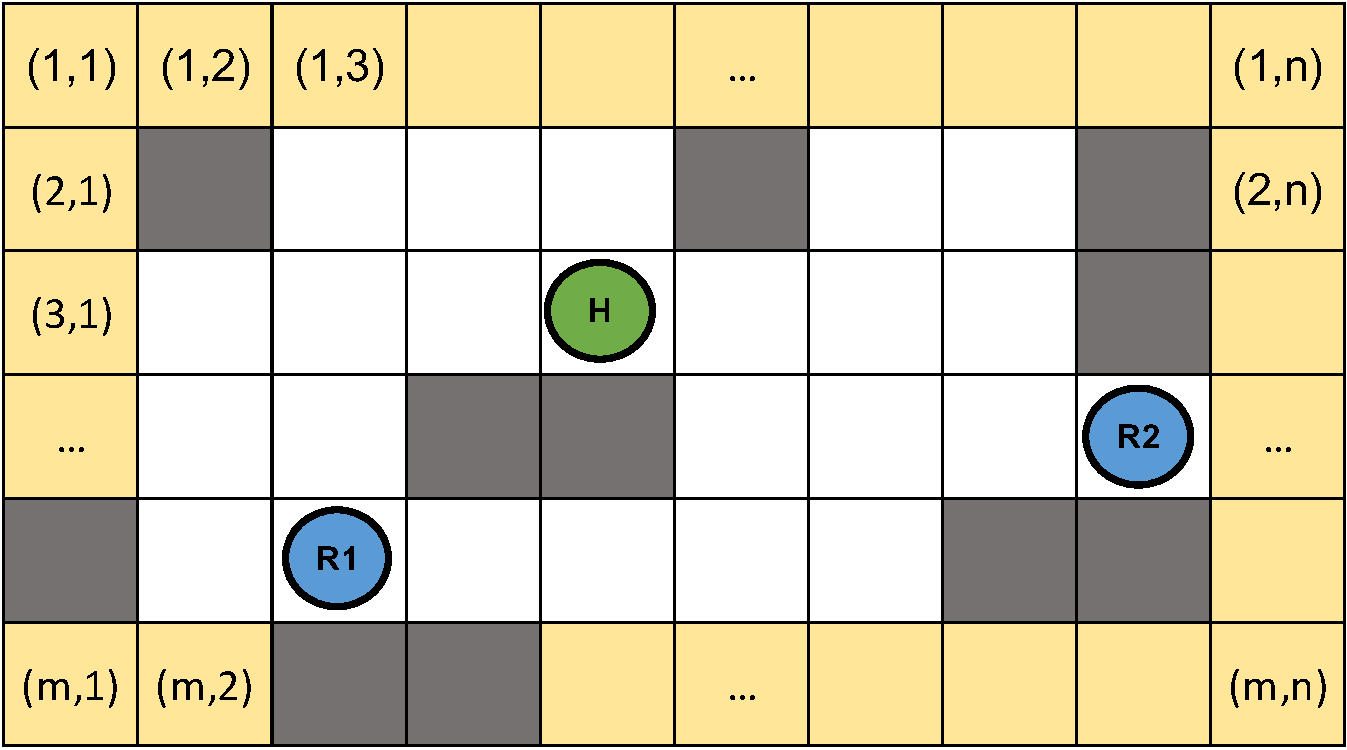
\includegraphics[width=0.5\columnwidth]{chase_map.pdf}
  	\caption{Rectangular field for \textit{Catch the Human} game.}
  	\label{fig:map}
  \end{figure}
  
  Develop an efficient algorithm with the following input and output:
  
\textbf{Input}
  	\begin{itemize}
  		\item values of \texttt{m} and \texttt{n}
  		\item coordinates of the initial squares for \textbf{H} as $(x_H,y_H)$, \textbf{R1} as $(x_{R1},y_{R1})$, and \textbf{R2} as $=(x_{R2},y_{R2})$ with $x\in\{1,n\}$ and $y\in\{1,m\}$
  		\item a list of coordinates of inaccessible (grey) squares
  	\end{itemize}

\textbf{Output}
\begin{itemize}
\item Output \textbf{True} if \textbf{H} can declare a yellow square
  \textbf{Y} such that \textbf{H} is able to escape.
  If there is no such \textbf{Y}, output \textbf{False}.
\end{itemize}

\textbf{Assumptions}
\begin{itemize}
\item Inaccessible squares are placed in a way that it is possible to move from any free square to any other free square in the field
\end{itemize}

Describe and design your algorithm by answering the following questions:
\begin{enumerate}[(a)]
\item Describe how to construct a graph to solve this problem. 
More precisely, describe the detailed procedure of creating the adjacency list of the graph from the given input. 
Clearly indicate which data structures you use. 
Analyse the runtime of your graph construction procedure.

\item Given the graph that is constructed in Part 3a, how do you
  efficiently determine whether \textbf{H} can escape? 
Describe your algorithm in concise (but precise) English, and analyse its runtime.
\end{enumerate}

\program

\item \textbf{Around the World Trip [total: 12]}
You are planning an around-the-world trip with your two best friends for the summer. 
There is a total of $n$ cities that the three of you want to visit.
As you are traveling around the world, you are worried about time zones and airport access. Therefore, some cities can only be visited after visiting another city first, which is in a nearby timezone or has an airport, which are expressed as a list of pairs (cityX,cityY) (cityX can only be visited after visiting cityY).

Given the total number of cities and a list of dependency pairs, is it possible for you all to visit all cities?

Your task is to write the function \verb|can_visit_all_cities|, which determines whether visiting the $n$ cities is possible or not given the dependencies. \textbf{(8 points)}

\textbf{Requirements}
\begin{itemize}
\item Your code must be written in Python 3, and the filename must be \verb|cities.py|.
\item We will grade only the \verb|can_visit_all_cities| function; please do not change its signature in the starter code. include as many helper functions as you wish.
\item You are {\bf not} allowed to use the built-in Python dictionary or set.
\item To get full marks, your algorithm must have average-case runtime
  $\mathcal{O}(m + n),$ where $m$ is the number of dependencies given.
\end{itemize}

\textbf{Input/Output Specification}
Please see the python starter code for input / output
specifications. 

\textbf{Write-up (4 points)}: in your \verb|ps3.pdf/ps3.tex| files,
include the following: an explanation of how your code works,
justification of correctness, and justification of desired
$\mathcal{O}(m + n)$ average-case runtime.

 \end{enumerate}

\end{document}

%%% Local Variables:
%%% mode: latex
%%% TeX-master: t
%%% End:
